\section{Introduction}

Unmanned aerial vehicles capable of vertical takeoff and landing have undergone a big boom in past few years. It is mainly thanks to arrival of multirotor helicopters (multicopters). Their capabilities span from being a platform for professional film makers, to toys and hobby products, up to military vehicles built for reconnaissance. These vehicles (fig. \ref{fig:quadru1}) have characteristically several propellers (typically four and more) with fixed pitch angle. The machine's mechanical design is usually simple by comparison with a classical helicopter. From the mechanical point of view it has several brushless motors with propellers mounted directly on them. There is a rigid body with utility platform, motor mounts and landing gear. They can operate in situations where the presence of a person could be hazardous (natural disasters) or they can help with work tasks which would otherwise require a very expensive solution e.g. inspection of high-voltage lines. They also find an application in situations where prior technology would not help --- archaeological imaging from low-to-mid altitude.

In most cases such aircraft requires a human operator to fly although it can offer a certain level of automatic assistance. Nowadays the global position system (GPS) receiver is embedded literally in every mobile phone thus it is no surprise that it can help with control of an unmanned aircraft (UAV) when flying outdoors. Commercially available platforms can assist with position hold or even fly to a particular location. Such technology can provide an automatic flight with precision up to $1 \jed{m}$ depending on the GPS, external conditions and the vehicle itself. The scientific community showed that there are methods to increase the precision of UAV control up to centimeters by using a better localization system than GPS (namely Vicon\footnote{Vicon system is based on multiples cameras capturing the object. http://www.vicon.com/}) and implementing advanced algorithms for automatic control \citep{brescianini2013polearobatics, kumar2010grasp}.

\begin{figure}[h]
\centering
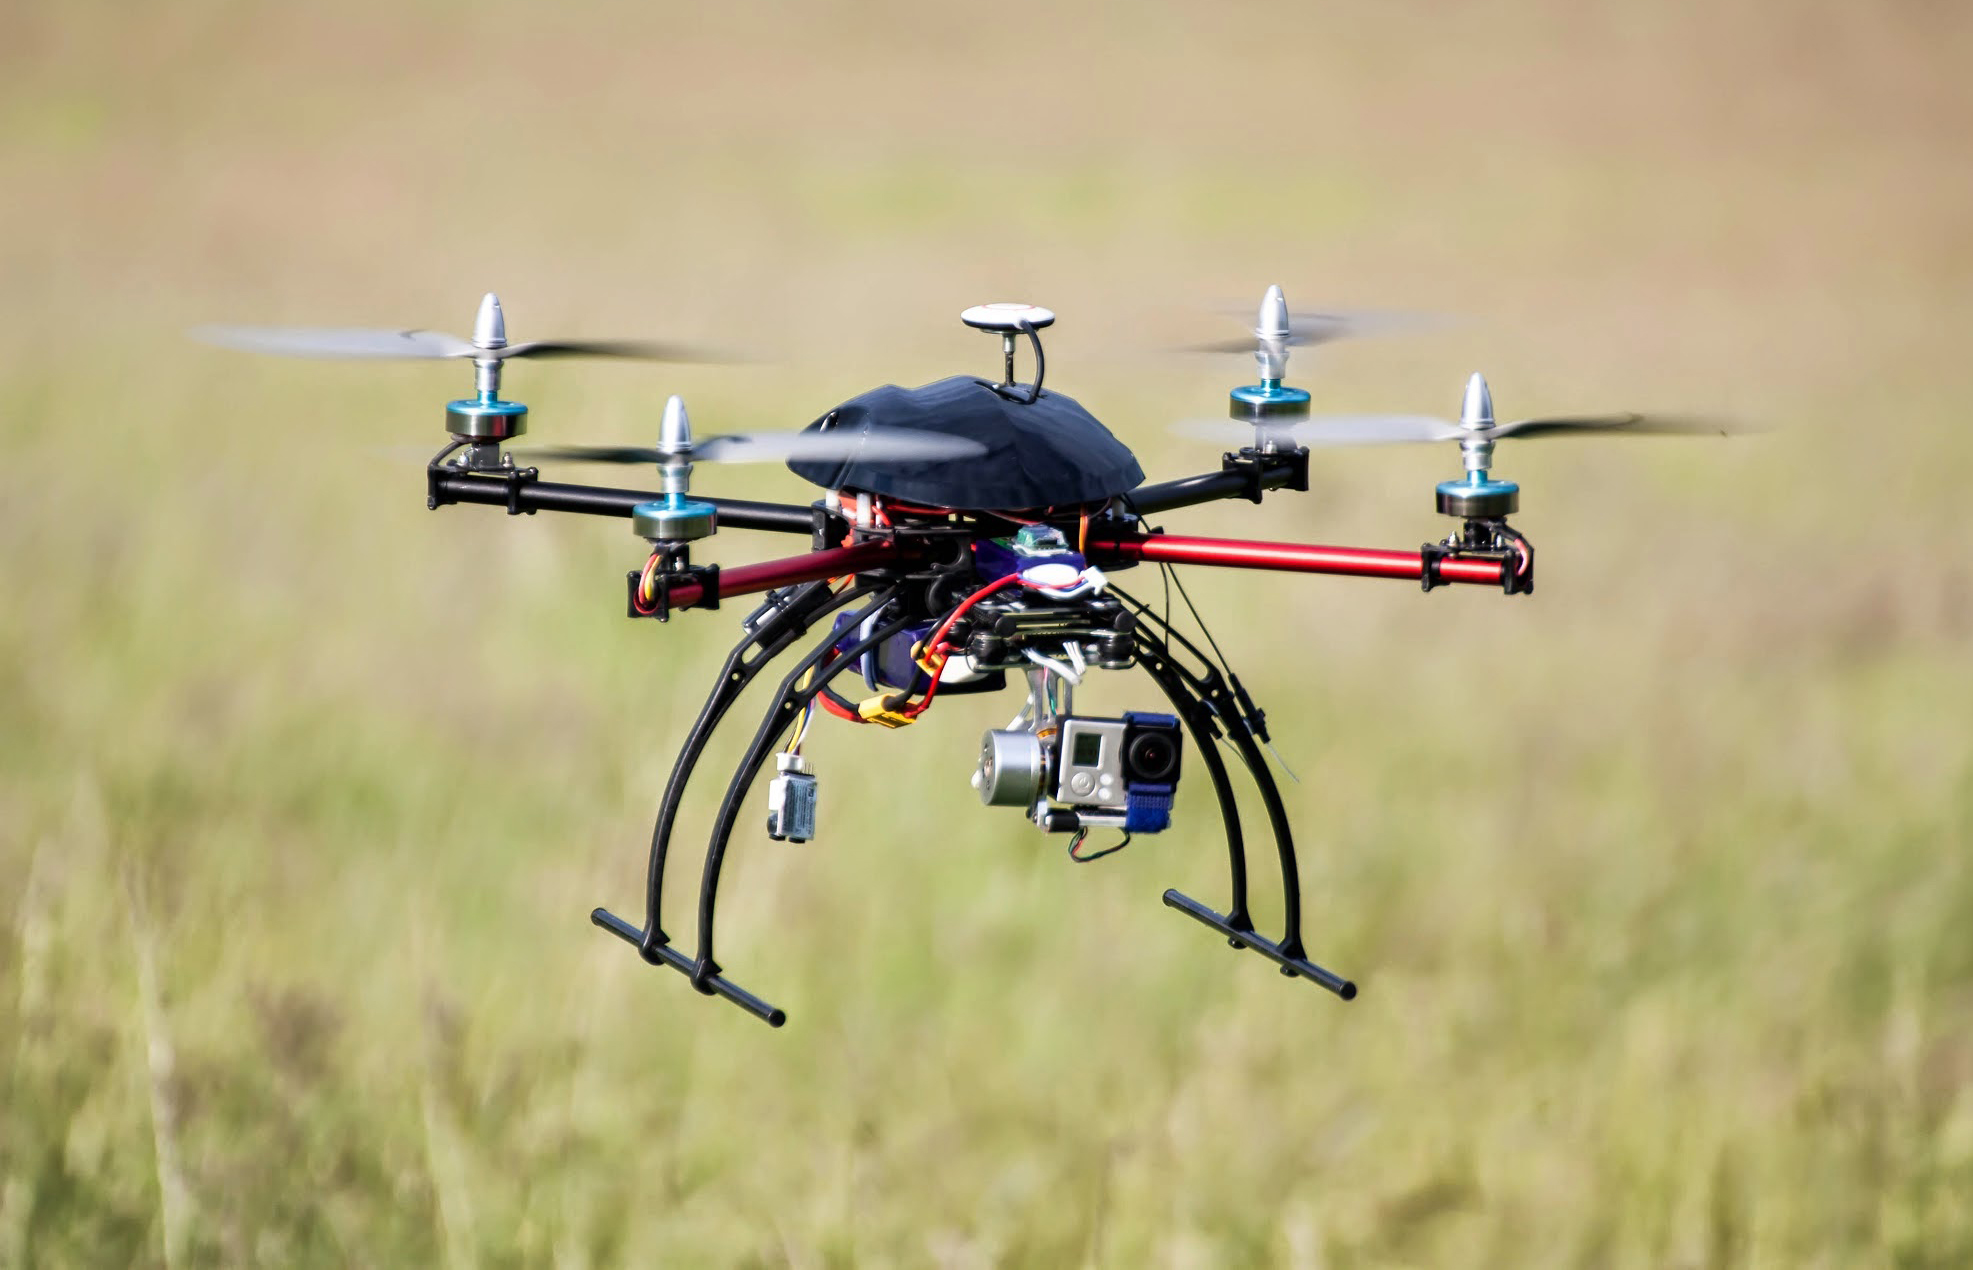
\includegraphics[width=0.75\textwidth]{fig/quadru1.jpg}
\caption{An example of multirotor aircraft used for aerial imaging.}
\label{fig:quadru1}
\end{figure}

Although previously mentioned work required an expensive laboratory hardware and on the ground computational power, it can be used as an example of what one could imagine an ''automatic assistance'' would be capable of when flying indoors. Since the multirotor UAV is a highly unstable machine (it will fly away when not controlled) there is feedback control necessary to even only stop it in the air. UAVs have been a subject of research for a long time. There is a current one with intention to build an automatic UAV that is supposed to work not only in a laboratory but also in uncontrolled indoor environment \citep{alexis2014rmpc}. It may seem that a modification of current outdoor solutions could be made but in practice it brings in new challenges and requires different approaches. The main ones are requirement of high precision control when flying indoors while omitting external localization system (like Vicon and GPS) and managing all computations onboard the vehicle itself.

The control mechanism used in today control systems is usually satisfactory when the precision is roughly defined by the GPS localization and the control settling time is slow. It is often narrowed to PID (proportional-integral-derivative controller) that is relatively easy to compute on common embedded hardware \cite{pixhawk, ardupilot}. But when increasing requirements on precision and settling time, such approach seems to suffer when controlling this kind of unstable vehicle (see prior work in chapter \ref{cap:prior_work}). Also when imposing a requirement not only to stabilize the vehicle (stop it   from moving) but to fly through a desired space trajectory, the need for a better control design approach emerges.

One of them is a model predictive control (MPC) which is a method based on the knowledge of a dynamical model of the controlled system. It formulates the computation of control actions as a mathematical optimization problem. Mathematical optimization can solve such problems by finding a minimum of a mathematical function. MPC uses a general prediction of system's future states to formulate the objective function to be optimized. There are various types of optimization problems based on the shape of the objective function and the range of its parameters. MPC is usually formulated as a continuous optimization with a convex quadratic objective function where the function itself penalizes squares of deviations from a desired state trajectory. When the optimum is found it guarantees that control actions will lead to an optimal future trajectory with respect to the objective function.

There are several important features that set the MPC apart from other control techniques such as PID. Firstly it works with the state space representation of the system and all states (e.g. position, velocity, acceleration, ...) participates as an input for the optimization, not only a control error of the tracked state (usually position) as it is with the PID. Although there are methods for nesting multiple controllers, the MPC offers a direct way to work with all states of the system. The other important feature is the way in which MPC handles constraints. We can impose constraints on inputs, systems states and even more complex ones. Though the optimization task becomes more complicated --- linearly constrained convex quadratic optimization, it still has a global optimum which can be found in reasonable time. Another feature is a capability to account in disturbances. When properly modeled and estimated, a disturbance can be used directly by the controller to produce adequate control actions.

As it was previously mentioned, MPC has been already successfully used for control of UAVs. But challenging task is to implement it solely on the hardware of the UAV where computational power is very limited. Today $\mu$-controllers\footnote{A microcontroller is an integrated circuit containing a processor, operating memory, program memory and peripheral controller.} can have parameters similar to $\approx 200 \jed{MHz}$ clock, $\approx 200 \jed{KB}$ RAM and mainly floating point performance in order of $10^7$ operations per second. Surely one could ask, why not to equip the UAV with a dedicated (miniaturized) PC to handle the computation. Our goal is to create a small all-in-one solution which can be mounted on any micro aerial vehicle (MAV) where the potential payload capacity could be only in hundreds of grams. In the long term this would allow to create a swarm of self-sustained MAVs that could solve tasks as remote sensing, localization of dangerous objects or mapping even in indoor and unknown environment.

\subsection{Problem statement}

Let us have a controllable multirotor UAV. The task is to design, build and implement an embedded controller that will utilize the model predictive control approach to drive the aircraft in a way suitable for indoor use and application, supporting precise trajectory following and future use in formations and swarms of helicopter. It entails a design and creation of dedicated circuit board which will allow to work with any usual UAV and extend its capabilities to fulfill other eventual robotic tasks. It should support connecting a variety of external peripherals and sensors to localize the helicopter in space. Firstly the system modeling and identification step need to be done to supply a dynamical model for simulation purposes and the MPC itself. It is followed up by a design of a state observer to track the current position of the UAV based on its sensors and to estimate all other states for purpose of the MPC. The design of the model predictive controller requires a formulation of optimization task

\begin{equation}
\label{eq:qmpc_intro}
\begin{aligned}
& \min_{\textbf{x} \in \mathbb{R}^{N}}
& & \mathrm{J}(\textbf{x}) = \frac{1}{2}\textbf{x}^T\textbf{H}\textbf{x} + \textbf{x}^T\textbf{c}\\
& \text{s.t.}
& & \text{constrains on \textbf{x}}
\end{aligned}
\end{equation}

where \textbf{x} is the solution that leads to the desired control actions over a certain \emph{prediction horizon}. A proper method for solving the optimization need to be chosen and implemented on the embedded hardware of the UAV. Previously mentioned tasks should be accompanied by simulation of the system including modeling of measurements, data filtration and the flight itself. There are minor tasks tied to the implementation and hardware design, mainly resolving communication, signal processing, data handling. The final outcome should be verified using variety of experiments testing its capabilities and finally compared to the prior solution used in the laboratory up to now.

\subsection{Previous work}
\label{cap:prior_work}

There has been a research on UAV control in laboratory of Intelligent and Mobile Robotics (IMR) group at FEE CTU Prague since 2011. The main focus has been in simulation of relatively localized UAV swarms and formations. Because it was also desired to verify the results experimentally, a development of hardware platform started. The first experiments has been done with AR Drone platform \citep{kranik2012drone} but it was shown that there is a need for a customizable platform capable of lifting heavier payload.

The first iteration of creating the custom platform is depicted in \citep{baca2013}. A custom control board was developed accommodating PID controllers. It could be mounted on a general purpose UAV and allowed connecting a dedicated onboard camera localization system \citep{faigl2013low}. Experiments showed that the UAV is able to track and follow the position of a ground robot marked for image recognition. It was also tested that localization based solely on the position of a moving object (another robot or UAV) tends to destabilize the vehicle. Experiments were conducted with a heterogeneous formation of two helicopters and one ground robot.

Subsequent work has been done in \citep{endrych2014} utilizing the same hardware accompanied by the \textit{px4flow} optical flow sensor. PID controllers were fine-tuned and the system was further improved to allow automatic flight even when the tracked object cannot be seen. This allowed creating formations of multiple UAV's which was not successful with former system. Experiments were again conducted to test the system's performance.

Furthermore, the need for a precise execution of indoor experiments led to increasing focus in development of the control system itself. This thesis describes a development of new hardware platform which satisfies demands that arose during previous work. The system should be capable of executing a MPC controller, transmitting telemetry to ground station as well as logging data onboard in realtime. 

\subsection{Related work}

It is difficult to find results on completely embedded MPC control of UAV. Those who are not only scientifically active in simulating flight control but verify their outcomes experimentally tend to use an external localization system and on the ground computational power, since it makes experiments much less demanding on particular hardware implementation. Following survey contains the state of the art of both, embedded and ground computed MPC.

The paper \citep{bangura2014realtimempc} shows an onboard quadratic implementation of MPC running on Pixhawk platform \citep{pixhawk}. Their unconstrained formulation solves the control problem with the prediction horizon of length 5 steps. Their UAV is supplied with position data gathered from the Vicon system and transmitted to the vehicle wirelessly. There are experiments evaluations which show that the vehicle is capable of tracking position step changes and harmonic trajectory.

The paper \citep{alexis2014rmpc} is considered as the current state of the art in the field of embedded MPC implementation on UAV. They have proposed a solution based on RMPC (Robust MPC)  utilizing an explicit formulation of the optimization task. The RMPC takes a form of a linear objective subject to linear constraints (Linear Programming). Their formulation allows a disturbance rejection which is demonstrated by experiments where the UAV follows a trajectory while being under the influence of wind gusts. Their experimental platform consists of two vehicles equipped with Atom based PC, one of them being localized by Vicon, the other one equipped with a ultrasonic rangefinder and camera for computing an optical flow. Their solution also allows to incorporate a collision avoidance directly into the control loop which is also experimentally verified in the paper.

Another work \citep{papachristos2013} (prior to \citep{alexis2014rmpc}) shows an implementation of a quadratic MPC, embedded on tilt-rotor aircraft, utilizing onboard Atom based computer. The position of UAV is estimated from onboard sensor data. Their constrained formulation can handle state constraints and optimize over prediction horizon of 8 steps. Experiments were conducted in order to show its ability to track desired 3D trajectory and reject position disturbances.

Authors of technical report \citep{bouffard2012dtic} and later paper \citep{bouffard2012learning} managed to implement the explicit formulation of quadratic MPC using onboard Atom PC. They localize the helicopter using the Vicon system and use a learning based MPC to improve the performance of the system. Their experiments involved a helicopter catching a flying ball.

Journal \cite{suzuki2014collision} presents a non-linear MPC formulation allowing to control several miniature, single-rotor helicopters in collision-free way. They utilize an external camera localization system as well as ground computer station. They optimize over $2 \jed{s}$ prediction horizon. Their simulation result has been experimentally verified with one miniature helicopter.

University ETH in Zurich has a long tradition of research in a field of UAV control. Some of their videos of helicopter aerobatics has been commonly known even among general public. They have accomplished astounding achievements with UAVs with the Vicon system involved \citep{brescianini2013polearobatics, Augugliaro2013buildingstructures}. Their contribution to MPC is published in \citep{ethMueller2013mpc}, but just as previous ones, it relies on the external localization system as well as the PC ground station.

\subsection{Contribution}

We were able to develop a control system for UAV that allows the execution of quadratic MPC onboard the aircraft. It consists of a single board equipped with two microcontrollers, telemetry module and SD-card data logger. The system was tested with the \textit{px4flow} optical flow sensor, but allows connecting other sensors and modules. A custom implementation of QMPC controls the UAV with $2.2\jed{s}$ prediction horizon. The implementation allows to estimate system disturbances with Kalman filter and reject them directly with the controller. When flying in indoor environment the system is able to track desired trajectories with errors in order of centimeters. Experiments shown that the system is competitive with current state of the art solutions. It can be implemented into very small UAVs (5 inch propellers) to allow experiments with tight formation in indoor environment. Our contribution is summarized in following points:

\begin{itemize}
\item design of hardware platform specifically intended for UAV experiments
\item 
\end{itemize}

\subsection{Mathematical notation}

The table \ref{tab:notation} denotes the basic mathematical notation used in this thesis.

\begin{table}[h]
\centering
\begin{tabular}{ll}
\hline
Symbol & Description \\
\hline
lower or upper case letter, e.g. $n$, $N$ & a scalar \\
bold lowercase letter, e.g. \textbf{x} & a column vector \\ 
bold uppercase letter, r.g. \textbf{A} & a matrix \\
$\textbf{x}^T$, $\textbf{A}^T$ & vector and matrix transpose \\
underlined vector, e.g. \textbf{\underline{x}} & concatenated vectors $\left(\textbf{x}_1^T,\textbf{x}_2^T,...,\textbf{x}_n^T\right)^T$ \\
\textbf{I} & identity matrix \\
\textbf{1} & matrix of ones \\
$x^{(W)}$ & $x$ in coordinate system $W$ \\ 
$x_{[t]}$, $\textbf{x}_{[t]}$ & $x$, $\textbf{x}$ in the sample time $t$ \\
$\mathbb{R}$, $\mathbb{N}$ & set of real and natural numbers \\
\hline
\end{tabular}
\caption{Overview of mathematical notation.}
\label{tab:notation}
\end{table}

